\documentclass[a4paper]{article}
\usepackage[pdftex]{graphicx}
\usepackage[utf8]{inputenc}
\usepackage{enumerate}
\usepackage{amssymb}
\usepackage{icomma}
\usepackage{siunitx}
\sisetup{locale=DE}
\usepackage{tikz}
\usepackage{href-ul}
\hypersetup{
	colorlinks=true,
	linkcolor=blue,
	urlcolor=blue}
\usepackage{geometry}
\geometry{a4paper, top=15mm, left=15mm, right=15mm, bottom=15mm,
	headsep=10mm, footskip=12mm}

\begin{document}
	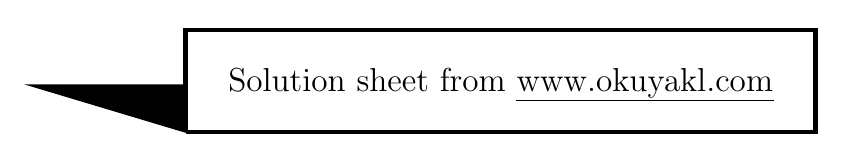
\begin{tikzpicture}(10,3)
		\draw[ultra thick](2,0) --(10,0) -- (10,1.3) --(2,1.3) -- (2,0);
		\draw[fill=black](2,0)-- (0,.6) -- (2,.6) -- (2,0);
		\node at (6,.6) {\large Solution sheet from \href{http://www.okuyakl.com}{www.okuyakl.com}};
	\end{tikzpicture}
	\vspace{0.5 cm}
	
	
	\noindent{\bf Task 1.}\\
	$t=\SI{0.70}{\second} \qquad v=\SI{3.7}{\meter\over\second}$
	\vspace{0.5 cm}
	
	\noindent{\bf Task 2.}\\
	$h=\SI{1,2}{\meter} + \SI{1,7}{\meter}=\SI{2,9}{\meter} \qquad E_{kin}=E_{pot}= \SI{18}{\joule}$
	\vspace{0.5 cm}
	
	\noindent{\bf Task 3.}\\
	$h=\SI{4,1}{\meter} \qquad t=\SI{1,8}{\second}$
	\vspace{0.5 cm}
	
	\noindent{\bf Task 4.}\\
	$h=\SI{160}{\kilo\meter}$\\
	There is no weightlessness during the acceleration and deceleration phases.
	This is the case during ascent during the burning period and during re-entry into the lower layers of the atmosphere.
	\vspace{0.5 cm}
	
	\noindent{\bf Task 5. a)}\\
	Potential energy = kinetic energy:
	$$
	\renewcommand{\arraystretch}{2}
	\begin{array}{rcll}
		
		m\cdot g \cdot h&=& 50\% \cdot {1\over 2}\cdot m \cdot v^2 &| :m \\
		g \cdot h &=& {1\over 4}\cdot v^2 &| :g \\
		h &=& {v^2 \over 4 \cdot g} \\
		h&=& {(\SI{11}{\meter\over \second})^2 \over 4\cdot \SI{9,81}{\meter\over \second^2}} & =\SI{3,1}{\meter}
	\end{array}
	$$
	$\Rightarrow$ the Spidercam is hit.
	\vspace{0.5 cm}
	
	\noindent{\bf Task 5. b)}\\
	Kinetic energy below = kinetic energy above + potential energy:
	$$
	\renewcommand{\arraystretch}{2}
	\begin{array}{rcll}
		E_{kin,bottom}&=&50\% \cdot {1\over 2}\cdot m \cdot v^2 + m\cdot g \cdot h \\
		&=& {1\over 4}\cdot \SI{0.42}{\kilogram} \cdot (\SI{11}{\meter\over \second})^2 + \SI{0.42}{ \kilogram} \cdot \SI{9.81}{\meter\over \second^2} \cdot \SI{2.4}{\meter} &=\SI{23}{\joule}
		
	\end{array}
	$$
	\vspace{0.5 cm}
	
	\noindent{\bf Task 5. c)}\\
	$$
	\renewcommand{\arraystretch}{2}
	\begin{array}{rcll}
		{1\over 2}\cdot m \cdot v_u^2&=&50\%\cdot {1\over 2}\cdot m \cdot v^2 + m\cdot g \cdot h &| :m\\
		{1\over 2} \cdot v_u^2&=&{1\over 4}\cdot v^2 + g \cdot h &| \cdot 2\\
		v_u^2&=&{1\over 2}\cdot v^2 + 2\cdot g \cdot h &| \sqrt{\qquad}\\
		v_u&=&\sqrt{{1\over 2}\cdot v^2 + 2\cdot g \cdot h} \\
		v_u&=&\sqrt{{1\over 2}\cdot (\SI{11}{\meter\over \second})^2 + 2 \cdot \SI{9,81}{\meter\over \second^ 2} \cdot \SI{2,4}{\meter}} &= \SI{10}{\meter\over \second}
	\end{array}
	$$
	\vspace{0.5 cm}
	
	\noindent{\bf Task 6. a)}\\
	$$E_{Span}={1\over 2}D\cdot s^2 ={1\over 2}\cdot \SI{7500}{\newton\over \meter}\cdot(\SI{0.40 }{\meter})^2 = \SI{0.60}{\kilo\joule}$$
	
	\newpage
	\noindent{\bf Task 6. b).}\\
	Potential energy = clamping energy
	$$
	\renewcommand{\arraystretch}{2}
	\begin{array}{rcll}
		
		m\cdot g \cdot h&=&{1\over 2}D\cdot s^2 &:(m\cdot g) \\
		h&=& {D\cdot s^2 \over 2\cdot m\cdot g }\\
		h&=& {\SI{7500}{\newton\over \meter}\cdot (\SI{0.40}{\meter})^2 \over 2\cdot \SI{75}{\kilogram} \cdot \SI{9.81}{\meter\over \second^2} } &= \SI{0.81}{\meter}\\
		h_w&=& h + \SI{4,0}{\meter} &= \SI{4,8}{\meter}
	\end{array}
	$$
	\vspace{0.5 cm}
	
	\noindent{\bf Task 6. c}\\
	Flight time = climb time + fall time
	$$
	\renewcommand{\arraystretch}{2}
	\begin{array}{rcll}
		
		t &=&t_s +t_f\\
		t &=& \sqrt{2\cdot h\over g} + \sqrt{2\cdot h_w\over g} \\
		t&=& \sqrt{2\cdot \SI{0.81}{\meter}\over \SI{9.81}{\meter\over \second^2} } + \sqrt{2\cdot \SI{ 4.8}{\meter}\over \SI{9.81}{\meter\over \second^2}}\\
		t&=& \SI{0.406}{\second} + \SI{0.989}{\second} &= \SI{1.4}{\second}
	\end{array}
	$$
	\vspace{0.5 cm}
	
	\noindent{\bf Task 7. a)}\\
	$$t= \sqrt{2\cdot l_s\over g} = \sqrt{2\cdot \SI{30}{\meter} \over \SI{9,81}{\meter\over \second^2} } = \SI{2,5}{\second}$$
	$$ v= \sqrt{2\cdot g \cdot l_s } = \SI{24}{\meter\over \second}$$
	\vspace{0.5 cm}
	
	\noindent{\bf Task 7. b)}\\
	Potential energy after = 60\% times potential energy before,
	measured by the total fall height \\
	$h_f=\SI{80}{\meter}-\SI{15}{\meter}=\SI{65}{\meter}$
	$$
	\renewcommand{\arraystretch}{2}
	\begin{array}{rcll}
		m\cdot g \cdot h^* &=& 0.60 \cdot m\cdot g \cdot h_f &|:(m\cdot g)\\
		h^* &=& 0.60 \cdot h_f \\
		h^* &=& 0.60 \cdot 65 &= \SI{39}{\meter}
	\end{array}
	$$
	For the height above ground $h_g$, the safety distance must be added to this, so:
	$$h_r=\SI{39}{\meter}+\SI{15}{\meter}=\SI{54}{\meter}$$
	\vspace{0.5 cm}
	
	
	\begin{minipage}{0.5\textwidth}
		\noindent{\bf Exercise 7. c)}\\
		Clamping energy = Potential energy:
		Elongation of the rope $s=\SI{80}{\meter}-\SI{30}{\meter}-\SI{15}{\meter}=\SI{35}{\meter}$
		$$
		\renewcommand{\arraystretch}{2}
		\begin{array}{rcll}
			
			{1\over 2}D\cdot s^2 &=& m\cdot g \cdot h_f &|\cdot 2|:s^2 \\
			D &=&{2 \cdot m\cdot g \cdot h_f \over s^2} \\
			D &=& {2 \cdot \SI{60}{\kilogram}\cdot \SI{9,81}{\meter\over \second^2} \cdot \SI{65}{\meter} \over ( \SI{35}{\meter})^2 } \\
			D &=& \SI{62}{\newton\over \meter}
			\end{array}
			$$
		\end{minipage}
	\hfill
\begin{minipage}{0.5\textwidth}
\begin{center}
\includegraphics[width=7 cm]{../../viecher/eendcomic.pdf}

Here you can go back to the \href{https://www.okuyakl.de/phys/p9frfL075/ae075.pdf}{task sheet}
\end{center}

\end{minipage}




\end{document}